\documentclass[12pt,letterpaper]{article}

\usepackage[protrusion=true,expansion=true]{microtype}  % Better typography
\usepackage{mathpazo}
\usepackage[T1]{fontenc}
\usepackage{setspace}
\usepackage[margin=1in]{geometry}
\usepackage{enumitem}
\usepackage{titlesec}
\usepackage[breaklinks]{hyperref}
\usepackage{tikz}
	\usetikzlibrary{positioning}
\usepackage{sidecap}

% For code samples
\usepackage{textcomp}
\usepackage{listings}
\usepackage{color}


% Import settings, which are stored in a separate file for convenience
% Syntax highlighting colors
\definecolor{lightgray}{rgb}{0.9, 0.9, 0.9}
\definecolor{darkgray}{rgb}{0.4, 0.4, 0.4}
\definecolor{purple}{rgb}{0.65, 0.12, 0.82}

\lstdefinelanguage{JavaScript}{
	keywords={break, case, catch, continue, debugger, default, delete, do, else, false, finally, for, function, if, in, instanceof, new, null, return, switch, this, throw, true, try, typeof, var, void, while, with},
	morecomment=[l]{//},
	morecomment=[s]{/*}{*/},
	morestring=[b]',
	morestring=[b]",
	ndkeywords={class, export, boolean, throw, implements, import, this},
	sensitive=true
}

\lstdefinestyle{js}{
	language=JavaScript,
	keywordstyle=\color{blue}\bfseries,
	ndkeywordstyle=\color{darkgray}\bfseries,
	identifierstyle=\color{black},
	commentstyle=\color{purple}\ttfamily,
	stringstyle=\color{red}\ttfamily,
	tabsize=2
}

\lstdefinestyle{html}{
	language=HTML,
	keywordstyle=\color{blue}\bfseries,
	ndkeywordstyle=\color{darkgray}\bfseries,
	identifierstyle=\color{black},
	commentstyle=\color{purple}\ttfamily,
	stringstyle=\color{red}\ttfamily,
	tabsize=4
}


% Set global defaults for code listings
\lstset{
	backgroundcolor=\color{lightgray},
	basicstyle=\singlespacing\footnotesize\ttfamily,
	breaklines=true,
	captionpos=b,
	extendedchars=true,
	showspaces=false,
	showstringspaces=false,
	showtabs=false,
	upquote=true
}


% All images will be in the img/ directory
\graphicspath{{./img/}}


% Sensible defaults for spacing and line breaks
\def\UrlBreaks{\do-\do_}
\titlespacing*{\section}{0pt}{0pt}{0pt}
\titlespacing*{\subsection}{0pt}{0pt}{0pt}
\doublespacing
\makeatletter


% Customize title
\renewcommand{\maketitle}{
	\begin{flushright}
		\@author\\\@date
	\end{flushright}
	\begin{center}
		{\LARGE\@title}
	\end{center}
}


% Set title
\title{\textbf{Angular vs. React}}
\author{William Gaul\\{ICS 419: Prof. Streveler}}
\date{\today}


\begin{document}
\maketitle

\renewcommand{\abstractname}{Executive Summary}
\begin{abstract}
	We are tasked with determining, non-destructively, whether an alien object is an artifact and/or intelligent. Philosophically, the nature of these concepts makes them extremely difficult, if not impossible, to test with empirical certainty. In this paper, we shall instead approach the problem mathematically. We first present easily testable definitions for ``artifact'' and ``intelligent'', then use these definitions to construct a set of appropriate tests.
\end{abstract}

\section{The Web, Then and Now}


%The modern web is inherently dynamic. As the Internet has evolved – as JavaScript plays an increasingly ubiquitous role and applications grow in size and complexity – developers have turned ever more toward web frameworks to make sense of the chaos. Many companies now favor applicants who have experience working with these frameworks, and so a good understanding of their usage and purpose is crucial. Why do they exist? What problems do they purport to solve, if any? How will they benefit developers and end users alike?
%This project aims to answer these questions by examining two very popular web frameworks in more detail: Angular and React. These frameworks were chosen in part for their popularity, but they also happen to take contrasting approaches to managing and abstracting application development. On the one hand, Angular offers an expressive extension of HTML specifically designed for dynamic views, centered on a concept called “two-way data binding.” On the other hand, React uses a component system that makes it easy to reason about application architecture, powered by “one-way data binding.”
%By evaluating both frameworks against a common baseline (tentatively, a simple example of DOM manipulation via a dropdown and input field), it is possible to gain a cursory understanding of their designs – that is, how they work and what they intend to do. More information can be gleaned from extensive documentation and numerous tutorials online; in particular, the Angular and React websites will reveal a great deal about goals and objectives. Although the purpose of this project is not to decide which framework is “better,” an appraisal of both frameworks on qualities such as “intuitive” and “testable” will be conducted, as it can be a helpful reflection of good application design in general.
%It is hoped that this project will inspire any budding web developers in the class to embrace web frameworks and the design principles that they afford. Moreover, as graduation approaches, studying this subject should be good preparation for entering the web development industry.



%~15 pages

%1. A well-chosen TITLE
%2. A brief Executive Summary (Abstract) of the Project
%3. A literature review of this topic (as appropriate)
%4. A written discussion of your project
%5. A discussion of any ethical issues you encountered while 
%researching or preparing your project
%6. A well-annotated bibliography of the references and materials 
%you used in the course of preparing your project
%7. A conclusion – What did you learn from all this?






\section*{Preliminary Definitions}

Call our object an \emph{agent}: ``something that acts in an environment'' \cite[p.~4]{Poole:2010}. Figure \ref{fig:AESystem} shows a visualization of the relationship between the agent and its environment.

\begin{SCfigure}[][h]
	\centering
	\caption{A very simplified view of an isolated agent-environment system. The agent impacts the environment through its actions, and is influenced by its perception of the environment.}
	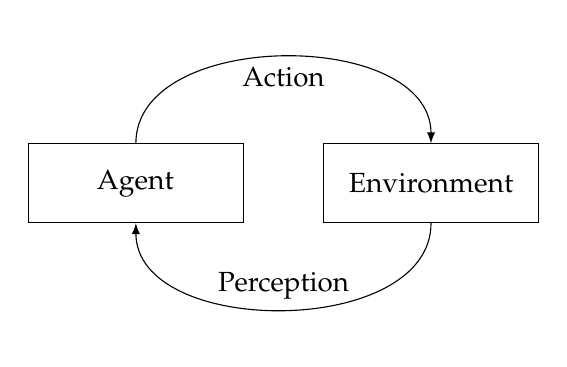
\begin{tikzpicture}[
		node distance=1.5cm and 1cm,
		ar/.style={->, >=latex},
		mynode/.style={draw, text width=2.5cm, minimum height=1cm, align=center}
	]
		\node[mynode] (agent) {Agent};
		\node[mynode,right=of agent] (env) {Environment};
		\draw[ar] (agent.north) to[out=90,in=90] node[below] {Action} (env.north);
		\draw[ar] (env.south) to[out=-90,in=-90] node[above] {Perception} (agent.south);
	\end{tikzpicture}
	\label{fig:AESystem}
\end{SCfigure}

For a given discrete moment $n$, the agent's behavior can be represented mathematically by the \emph{agent function} $f : P^\ast \to A_n$, which maps a history of inputs from the environment $P^\ast = \bigcup\limits_{i=1}^n P_i$ (the \emph{percept sequence}) to an output from the agent $A_n$ (an \emph{action}). The agent is simply some physical system running an implementation of this agent function \cite{Russell:2010}.

Every such action $A_n$ causes the environment to enter a new state, represented by the state function $g : S_{n-1}, A_n \to S_n$. The cycle begins anew when the agent perceives some subset of this new state $P_{n+1} \in S_n$. Finally, a notion of the environment's history is captured in the sequence of states $S^\ast = \bigcup\limits_{i=1}^n S_i$.

\section*{What is an Artifact? What is Intelligence?}

To simplify matters \footnote{It is common to think of an artifact as something ``made'' rather than ``born''. However, this definition is ambiguous and difficult to test. How would we characterize objects such as genetic clones? Another example: toasters are artificial because we make them, but what if we suddenly discovered a ``toaster tree'' deep in the Amazon jungle? \cite{CM317}.}, we define an \emph{artifact} to be an agent whose physical system is a digital computer. A \emph{digital computer} is a machine that implements an algorithm, or an ordered and finite set of precise, explicit, repeatable instructions \cite{Anderson:2006}. This is the same as saying that an artifact is an agent whose agent function is an algorithm. Note here that we are not concerned with the physical nature of the computer (e.g. that it runs on electricity or uses transistors) because such characteristics may not be observable.

Typically, intelligence is determined by evaluating either thought processes or behaviors against some established measure. For example, the Turing Test considers intelligence to be equivalent to behaving humanly. In this situation, the alien object cannot be evaluated against a human measure of intelligence -- rather, it must be evaluated against an ``ideal performance measure, called \emph{rationality}'' \cite[p.~1]{Russell:2010}. Likewise, we cannot base a test on its (possibly alien) thought processes, and so must rely entirely on observations of its behavior. Thus, an intelligent agent is defined here to be an agent that acts rationally.

We adopt the definition of a rational agent presented by Russell and Norvig \cite[p.~37]{Russell:2010}:

\begin{quote}
	\singlespacing
	For each possible percept sequence, a rational agent should select an action that is expected to maximize its performance measure, given the evidence provided by the percept sequence and whatever built-in knowledge the agent has.
\end{quote}

The \emph{performance measure} $q : S^\ast \to Q$ is a metric that attempts to quantify the desirability of $S^\ast$, and must be chosen wisely (``according to what one actually wants in the environment'') in order to successfully evaluate an agent's performance \cite[p.~37]{Russell:2010}. Thus, an intelligent agent is one whose agent function satisfies $\max_{A_n} q(S_{n-1}^\ast \cup g(S_{n-1}, A_n))$.

\section*{Establishing I/O}

It has been shown that in order for an object to be either an artifact or intelligent, it must implement an agent function. Thus, a necessary prerequisite for our tests is to establish the object's sensors and actuators -- that is, its input and output (I/O) channels. Once these channels have been established, they can be used to control the object's percept sequence and observe the object's actions.

This is an important step because nothing can be assumed about how the alien object interacts with its environment. Perhaps it communicates chemically or telepathically. Perhaps it vocalizes, but in an alien language (it almost certainly does not know English). Unfortunately, as with many first contact situations between human cultures, the task of establishing I/O is largely one of trial and error and can be a lengthy, gradual process \cite{Ivir:1991}. However, between human cultures there is the advantage that I/O channels and cognitive bounds are known in advance \footnote{That is, we can safely assume that the other party is \emph{capable} of both producing and understanding some form of language, and that this will be done using the ears and mouth (in terms of oral language).}, which does not exist in this situation.

It is therefore recommended that a variety of methods be used to communicate with the object initially. If any method elicits a response, take note of both the method and the observed response (i.e. how it was produced). Iterate, refining the input method until reliable communication is established -- ``reliable'' entails that there is statistically significant confidence that, given an input, the object will respond.

\section*{Artifact?}

If an object operates according to some algorithm, then it is an artifact.

Note that, in the general case, it is impossible to devise an algorithm to determine whether something else is an algorithm \cite{Weiss:2008}. Our test shall therefore be designed and described in a ``fuzzy'' manner. Indeed, given the lack of a precise set of instructions to carry out the test, some subjective determinations will have to be made about the nature of the object and its behavior.

Suppose that the object does operate according to an algorithm. Then we know the following to be true:

\begin{itemize}
	\singlespacing
	\item Given an input, the object must eventually produce output
	\item The object's behavior is \emph{deterministic}; given a particular input, the object will always produce the same output
\end{itemize}

Verifying whether the object eventually produces output is in the class of halting problems \cite{Russell:2010} that are not practically decidable \footnote{If the object \emph{does} produce output, but only after a million years, it is still considered finite \ldots but waiting a million years to complete a test is hardly advisable.}. For that reason, we advise restricting each I/O cycle to a reasonable interval (e.g. 5 minutes): if the object does not respond in that time, it has failed the test.

Consider that, when we interact with the object, we are really modifying the state of its environment $S_n$. Its response is then $A_{n+1} = f(P_n^\ast \cup P_{n+1})$, where $P_{n+1} \in S_n$; its behavior is dependent not only on some unknowable subset of the environment state $P_{n+1}$, but on all such past percepts $P_n^\ast$. To minimize the effects of these terms and maximize confidence in the outcome's validity, we propose the following test:

\begin{enumerate}
	\singlespacing
	\item Maintain a prediction function $p : I \to O$ that predicts the object's response $O$ to a given prompt $I$. $p$ may be adjusted to accommodate observed object behavior.
	\item Repeatedly prompt until, given $S_{n} \cup I$, it is observed that $O = A_{n+1}$.
	\item If it is observed above some reasonable confidence level (e.g. 95\%) that this trend continues, then we say $p$ approximates $f$: if $p$ is an algorithm, then we can say with reasonable confidence that $f$ is also an algorithm.
\end{enumerate}

\section*{Intelligent?}

If an object's actions maximize its performance measure, then it is intelligent.

Let $p : I \to O$ be a function chosen such that $I$ is an input capable of being transmitted to the object. Call a \emph{cycle} an I/O pair $(I, A_n)$. Then $q$ is the reciprocal of the number of cycles it takes until $O = A_n$. We propose the following test:

\begin{enumerate}
	\singlespacing
	\item\label{item:choose} Pick an arbitrary $I$ and set $n = 0$
	\item\label{item:again} Communicate $I$ to the object and increment $n$
	\item If $p(I) \neq A_n$, go to Step \ref{item:again}
	\item If $p(I) = A_n$, take a note of $n$ and go to Step \ref{item:choose}
\end{enumerate}

Informally, this test repeatedly prompts the object for $I$ until it produces the ``correct'' response $O$, then continues with a different input $I$. We evaluate its performance against the performance measure $q = \frac{1}{n}$. If the object is rational, then it should attempt to maximize $q$ by minimizing $n$, the number of cycles it takes to produce $O$ for a particular $I$, and over time we should see $n$ gradually decrease to $1$. Because in the negative case the test can continue interminably, we impose a loose bound on its length: if it cannot be decided whether $n$ is converging to some local minimum after 10 (or some other reasonably low number) unique inputs, then the object has failed and is not intelligent.

An interesting consequence of this test is that in order for an object to be considered rational, it must first learn $q$ (and by extension, $p$). This suggests that the ability to learn may be a necessary condition for intelligence, but we shall leave such a discussion for another time.

\section*{Future Work}

We have here presented a set of tests that we are reasonably confident will determine whether an alien object is an artifact and/or intelligent, but there is a lot of room for improvement. Future iterations of these tests may adopt more rigorous definitions or incorporate empirical feedback to increase their efficacy.

\newpage

\appendix
\section{Code Listings}

\subsection*{Pure JavaScript}

\lstinputlisting[style=html,caption={index.html},label={lst:pureHTML}]{../examples/pure-js/index.html}
\lstinputlisting[style=js,caption={app.js},label={lst:pureJS}]{../examples/pure-js/app.js}

\newpage

\subsection*{Angular}

\lstinputlisting[style=html,caption={index.html},label={lst:angularHTML}]{../examples/angular/index.html}
\lstinputlisting[style=js,caption={app.js},label={lst:angularJS}]{../examples/angular/app.js}

\newpage

\subsection*{React}

\lstinputlisting[style=html,caption={index.html},label={lst:reactHTML}]{../examples/react/index.html}
\lstinputlisting[style=js,caption={app.js},label={lst:reactJS}]{../examples/react/app.js}

\newpage

% BIBLIOGRAPHY (Note: We use a special version of IEEEtran that has sorting and annotations)
\begin{flushleft}
\begin{singlespace*}
	\bibliographystyle{./IEEEtran}
	\bibliography{angular-vs-react}
\end{singlespace*}
\end{flushleft}

\end{document}
